\documentclass[12pt]{article}
\usepackage{amsmath}
\usepackage{amssymb}
\usepackage[letterpaper,margin=0.85in,centering]{geometry}
\usepackage{fancyhdr}
\usepackage{enumerate}
\usepackage{lastpage}
\usepackage{multicol}
\usepackage{graphicx}

\reversemarginpar

\pagestyle{fancy}
\cfoot{}
\lhead{Math 2560}\chead{Worksheet \# 7}\rhead{Thursday 10\textsuperscript{th} March, 2016}
%\rfoot{Total: 10 points}
%\chead{{\bf Name:}}
\newcommand{\points}[1]{\marginpar{\hspace{24pt}[#1]}}
\newcommand{\skipline}{\vspace{12pt}}
%\renewcommand{\headrulewidth}{0in}
\headheight 30pt

\newcommand{\di}{\displaystyle}
\newcommand{\abs}[1]{\lvert #1\rvert}
\newcommand{\len}[1]{\lVert #1\rVert}
\renewcommand{\i}{\mathbf{i}}
\renewcommand{\j}{\mathbf{j}}
\renewcommand{\k}{\mathbf{k}}
\newcommand{\R}{\mathbb{R}}
\newcommand{\aaa}{\mathbf{a}}
\newcommand{\bbb}{\mathbf{b}}
\newcommand{\ccc}{\mathbf{c}}
\newcommand{\dotp}{\boldsymbol{\cdot}}
\newcommand{\bbm}{\begin{bmatrix}}
\newcommand{\ebm}{\end{bmatrix}}                   
                  
\begin{document}


%\author{Instructor: Sean Fitzpatrick}
\thispagestyle{fancy}
%\noindent{{\bf Name and student number:}}
The problems on this worksheet are for in-class practice during tutorial. You are free to collaborate and to ask for help. They don't count for course credit, but it's a good idea to make sure you know how to do everything before you leave tutorial -- similar problems may show up on a test or assignment.

\begin{enumerate}
 \item Evaluate the improper integral, or explain why it does not exist:
\begin{enumerate}
 \item $\di \int_0^\infty e^{4-3x}\,dx$
 \item $\di \int_{-\infty}^\infty \frac{1}{4+x^2}\,dx$
 \item $\di \int_{-\infty}^\infty \frac{x}{1+x^2}\,dx$
 \item $\di \int_1^\infty\frac{\ln x}{x^2}\,dx$
\end{enumerate}
 \item Find the area between the given curves:
\begin{enumerate}
 \item $y=x^2-3x+2$, and $y=-3x+3$
 \item $y=\sqrt{x}$, $y=-2x+3$, and $y=-\frac{1}{2}x$.
\end{enumerate}
\item Find the volume of the solid of revolution:
\begin{enumerate}
 \item Generated by revolving the region bounded by $y=x^2-2x+2$ and $y=2x-1$ about the $x$-axis.
 \item Generated by revolving the region bounded by $y=x^2-2x+2$ and $y=2x-1$ about the line $y=1$.
 \item Generated by revolving the triangle with vertices $(1,1), (1,2)$, and $(2,1)$ about the $y$-axis.
 \item Generated by revolving the triangle with vertices $(1,1), (1,2)$, and $(2,1)$ about the $x$-axis.
\end{enumerate}
\item Find the length of the curve $y=2x^{3/2}-\dfrac{1}{\sqrt{6}}\sqrt{x}$, for $0\leq x\leq 9$.
\item Find the area of the surface generated by revolving the the curve $y=x^2$, for $0\leq x\leq 1$, about the $y$-axis.
\item Find the area enclosed by the following regions:
\begin{enumerate}
 \item The region above the $x$-axis and below the spiral $r=\theta$, for $0\leq \theta \leq \pi$.
 \item The region given by the part of the first quadrant inside the curve $r=1+\sin\theta$.
 \item One loop of the curve $r=\sin 4\theta$.
 \item The inner loop of the curve $r=1+2\sin\theta$.
\end{enumerate}
\pagebreak

Diagrams for problem 6:
\begin{multicols}{2}
 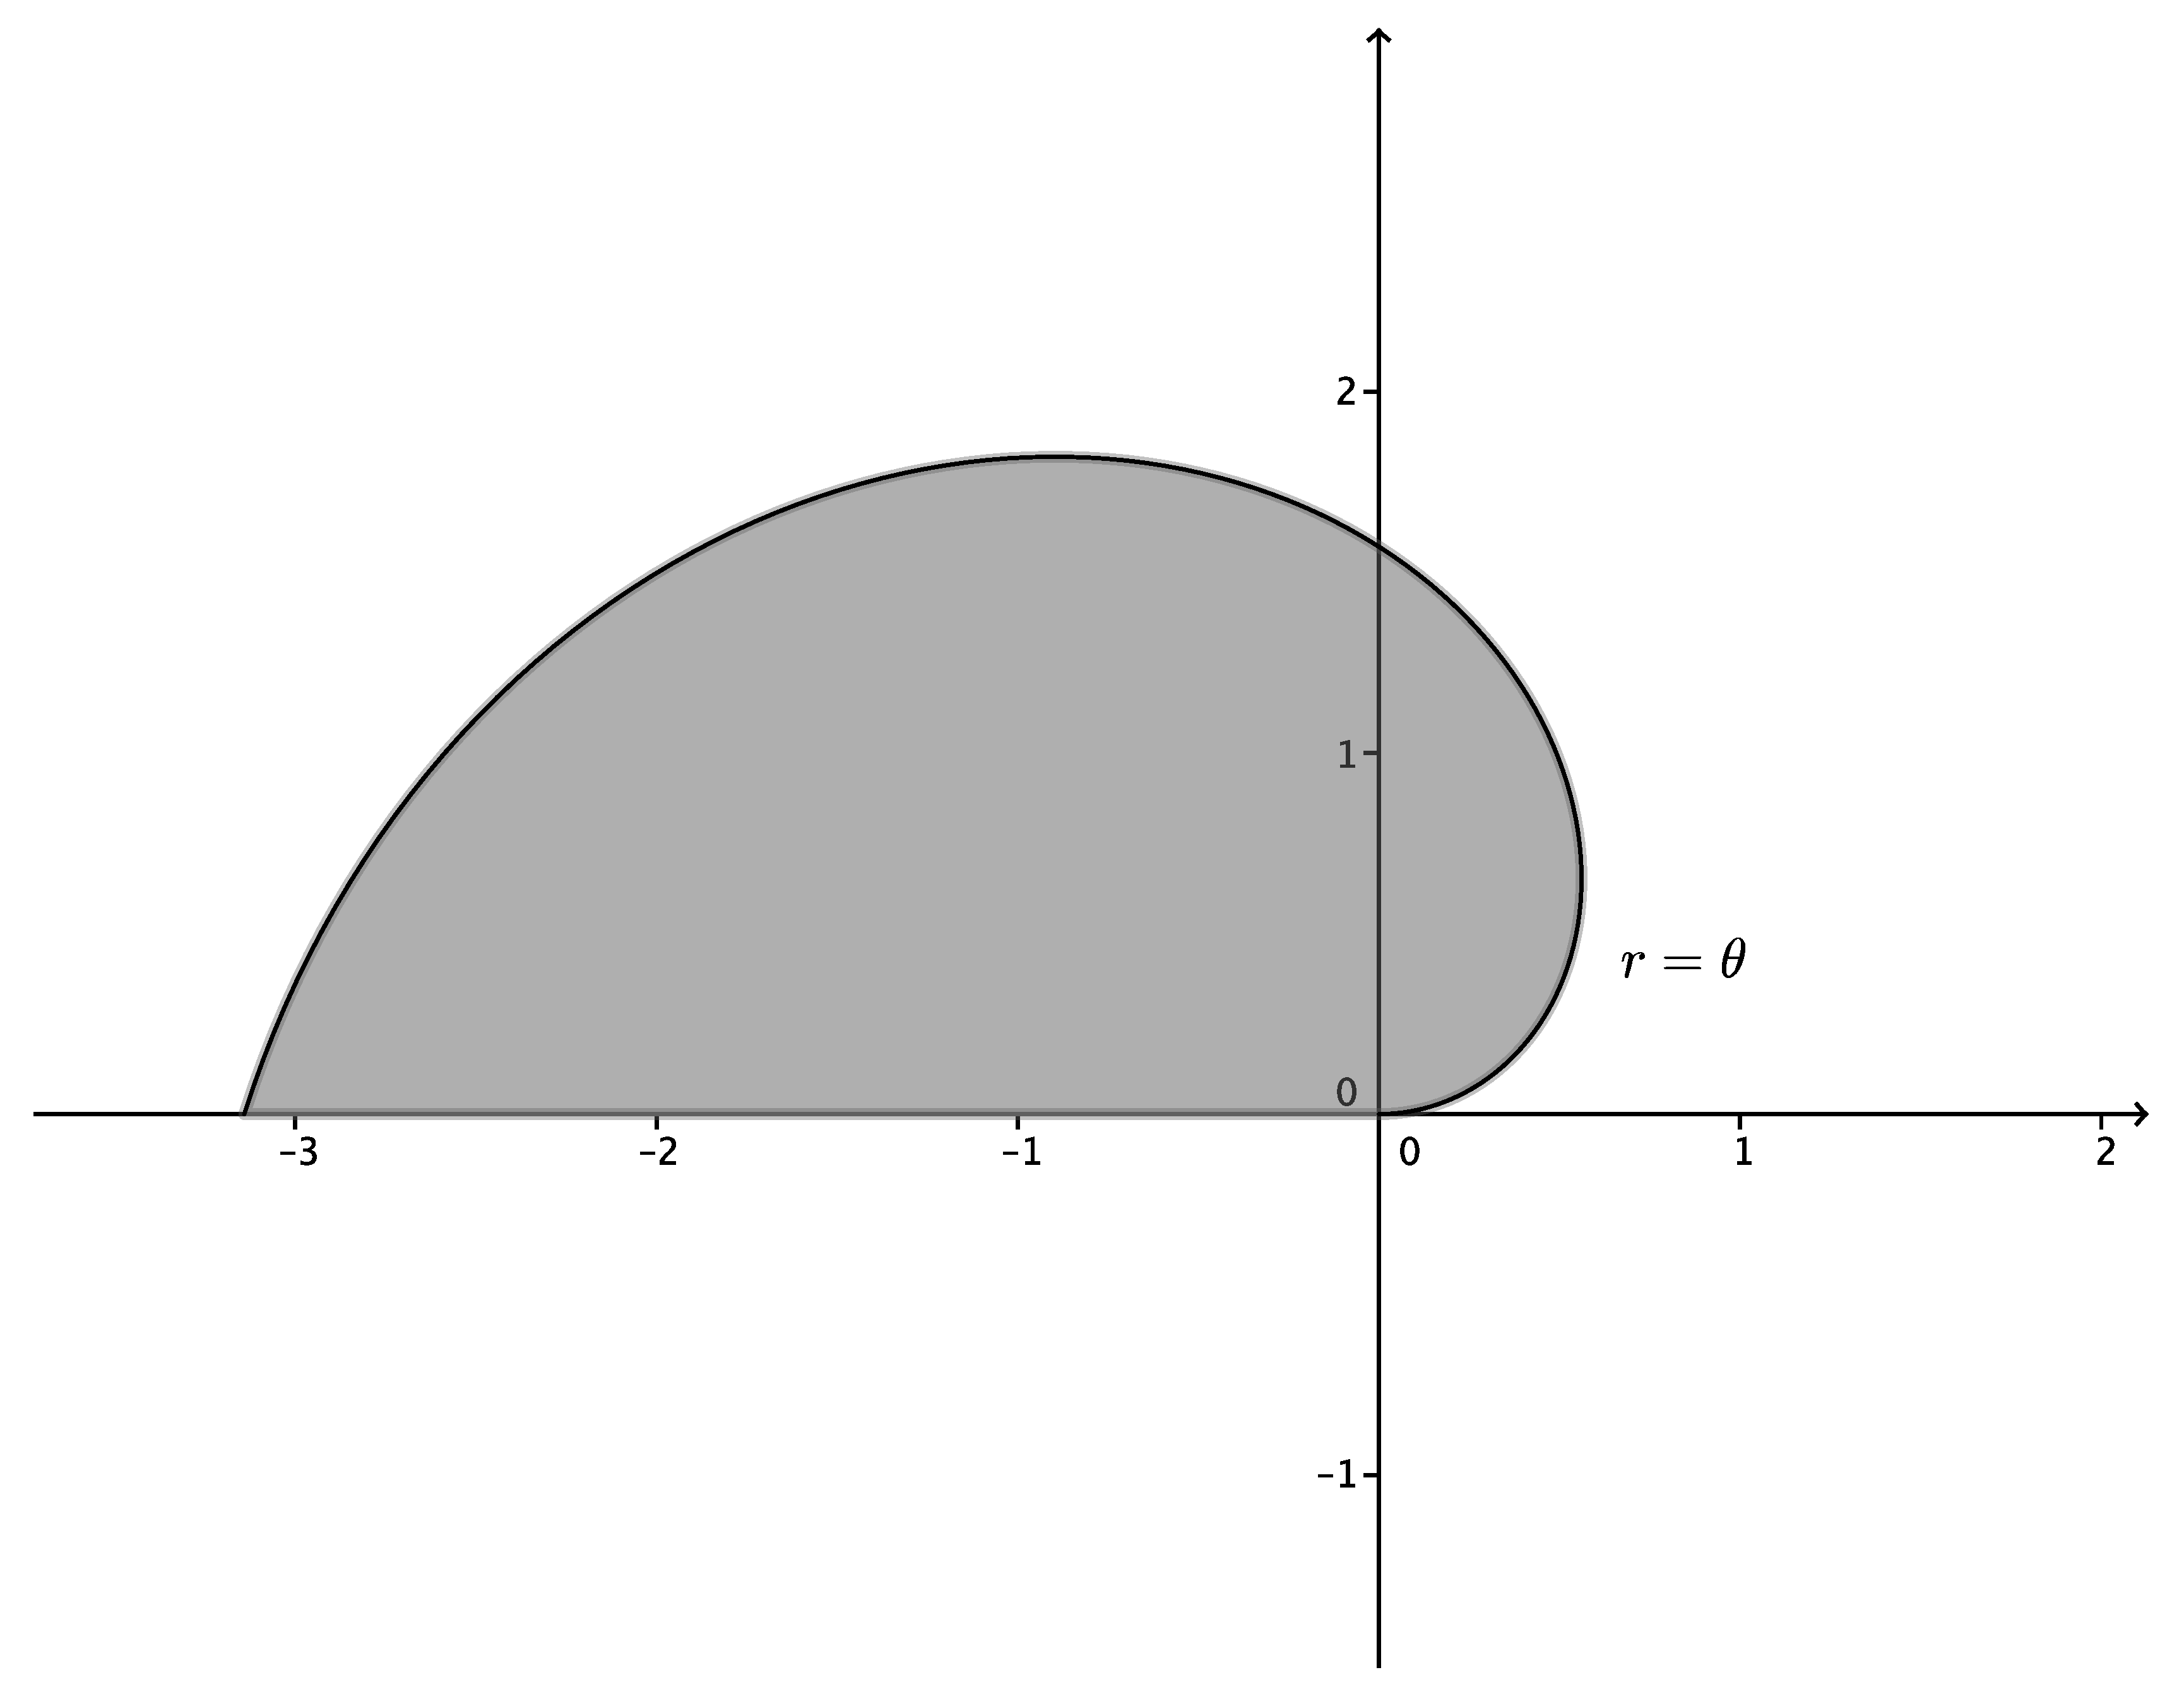
\includegraphics[width=0.9\columnwidth]{WS7-6a}

 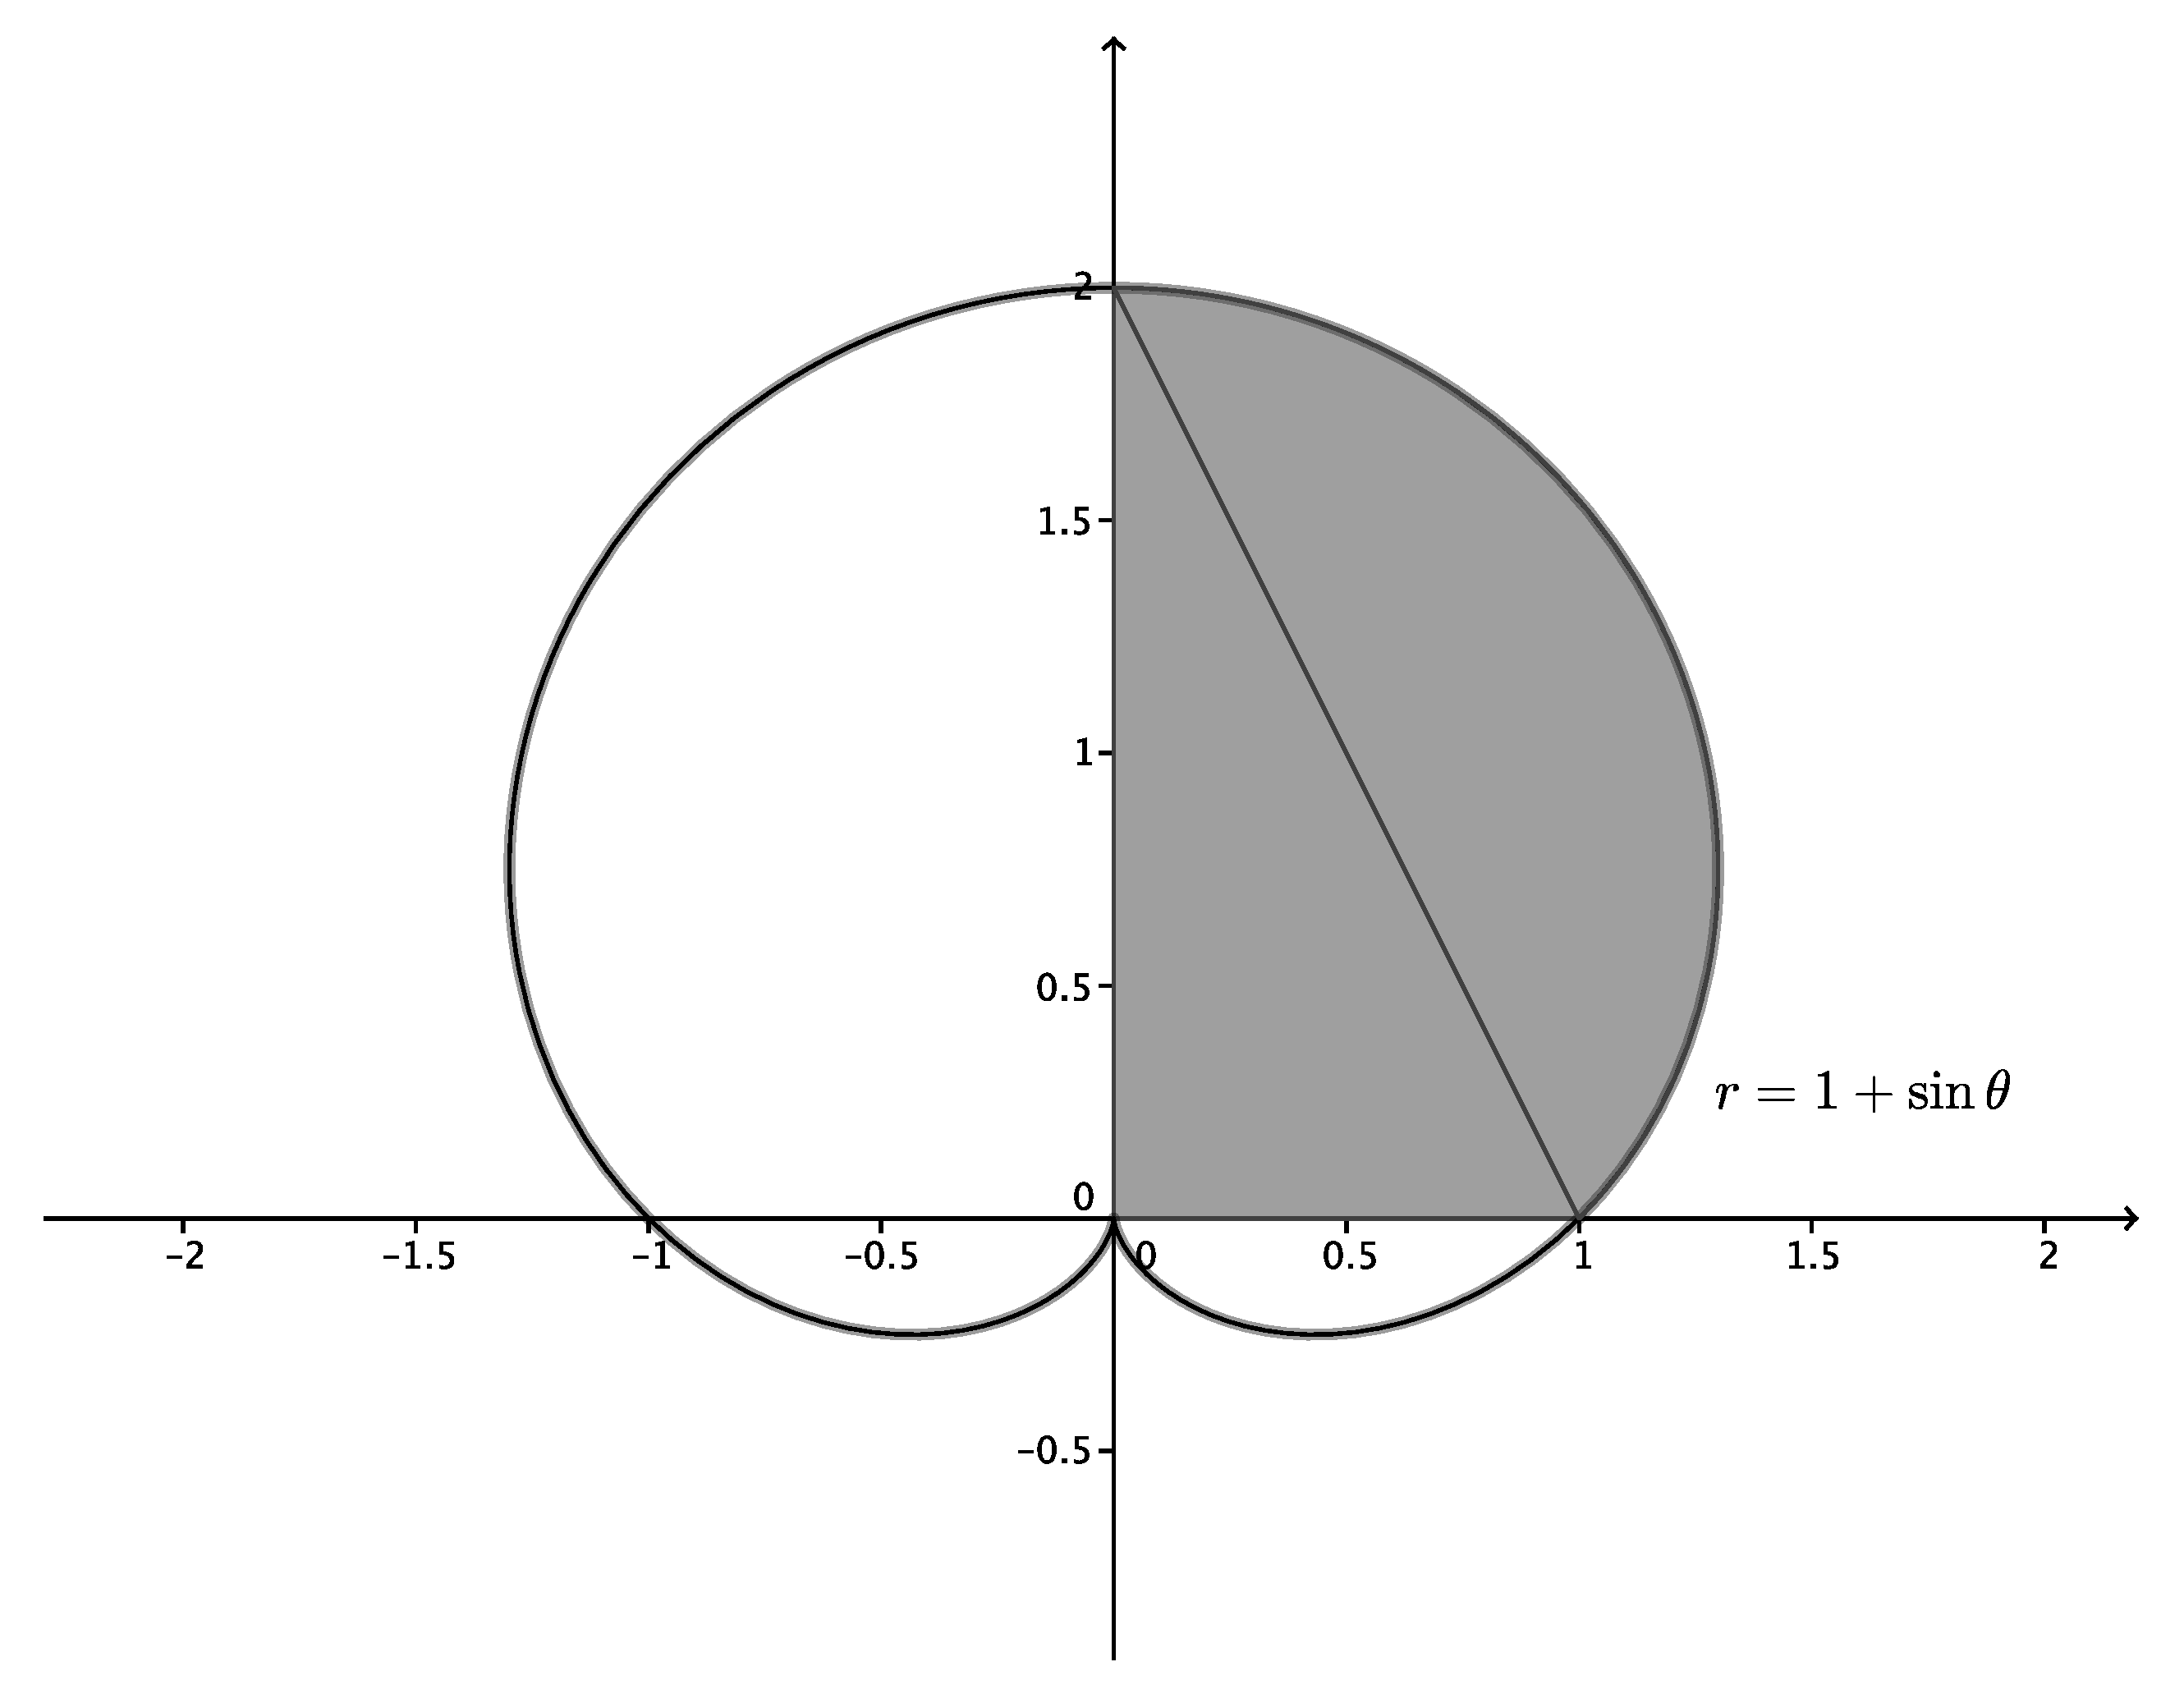
\includegraphics[width=0.9\columnwidth]{WS7-6b}

 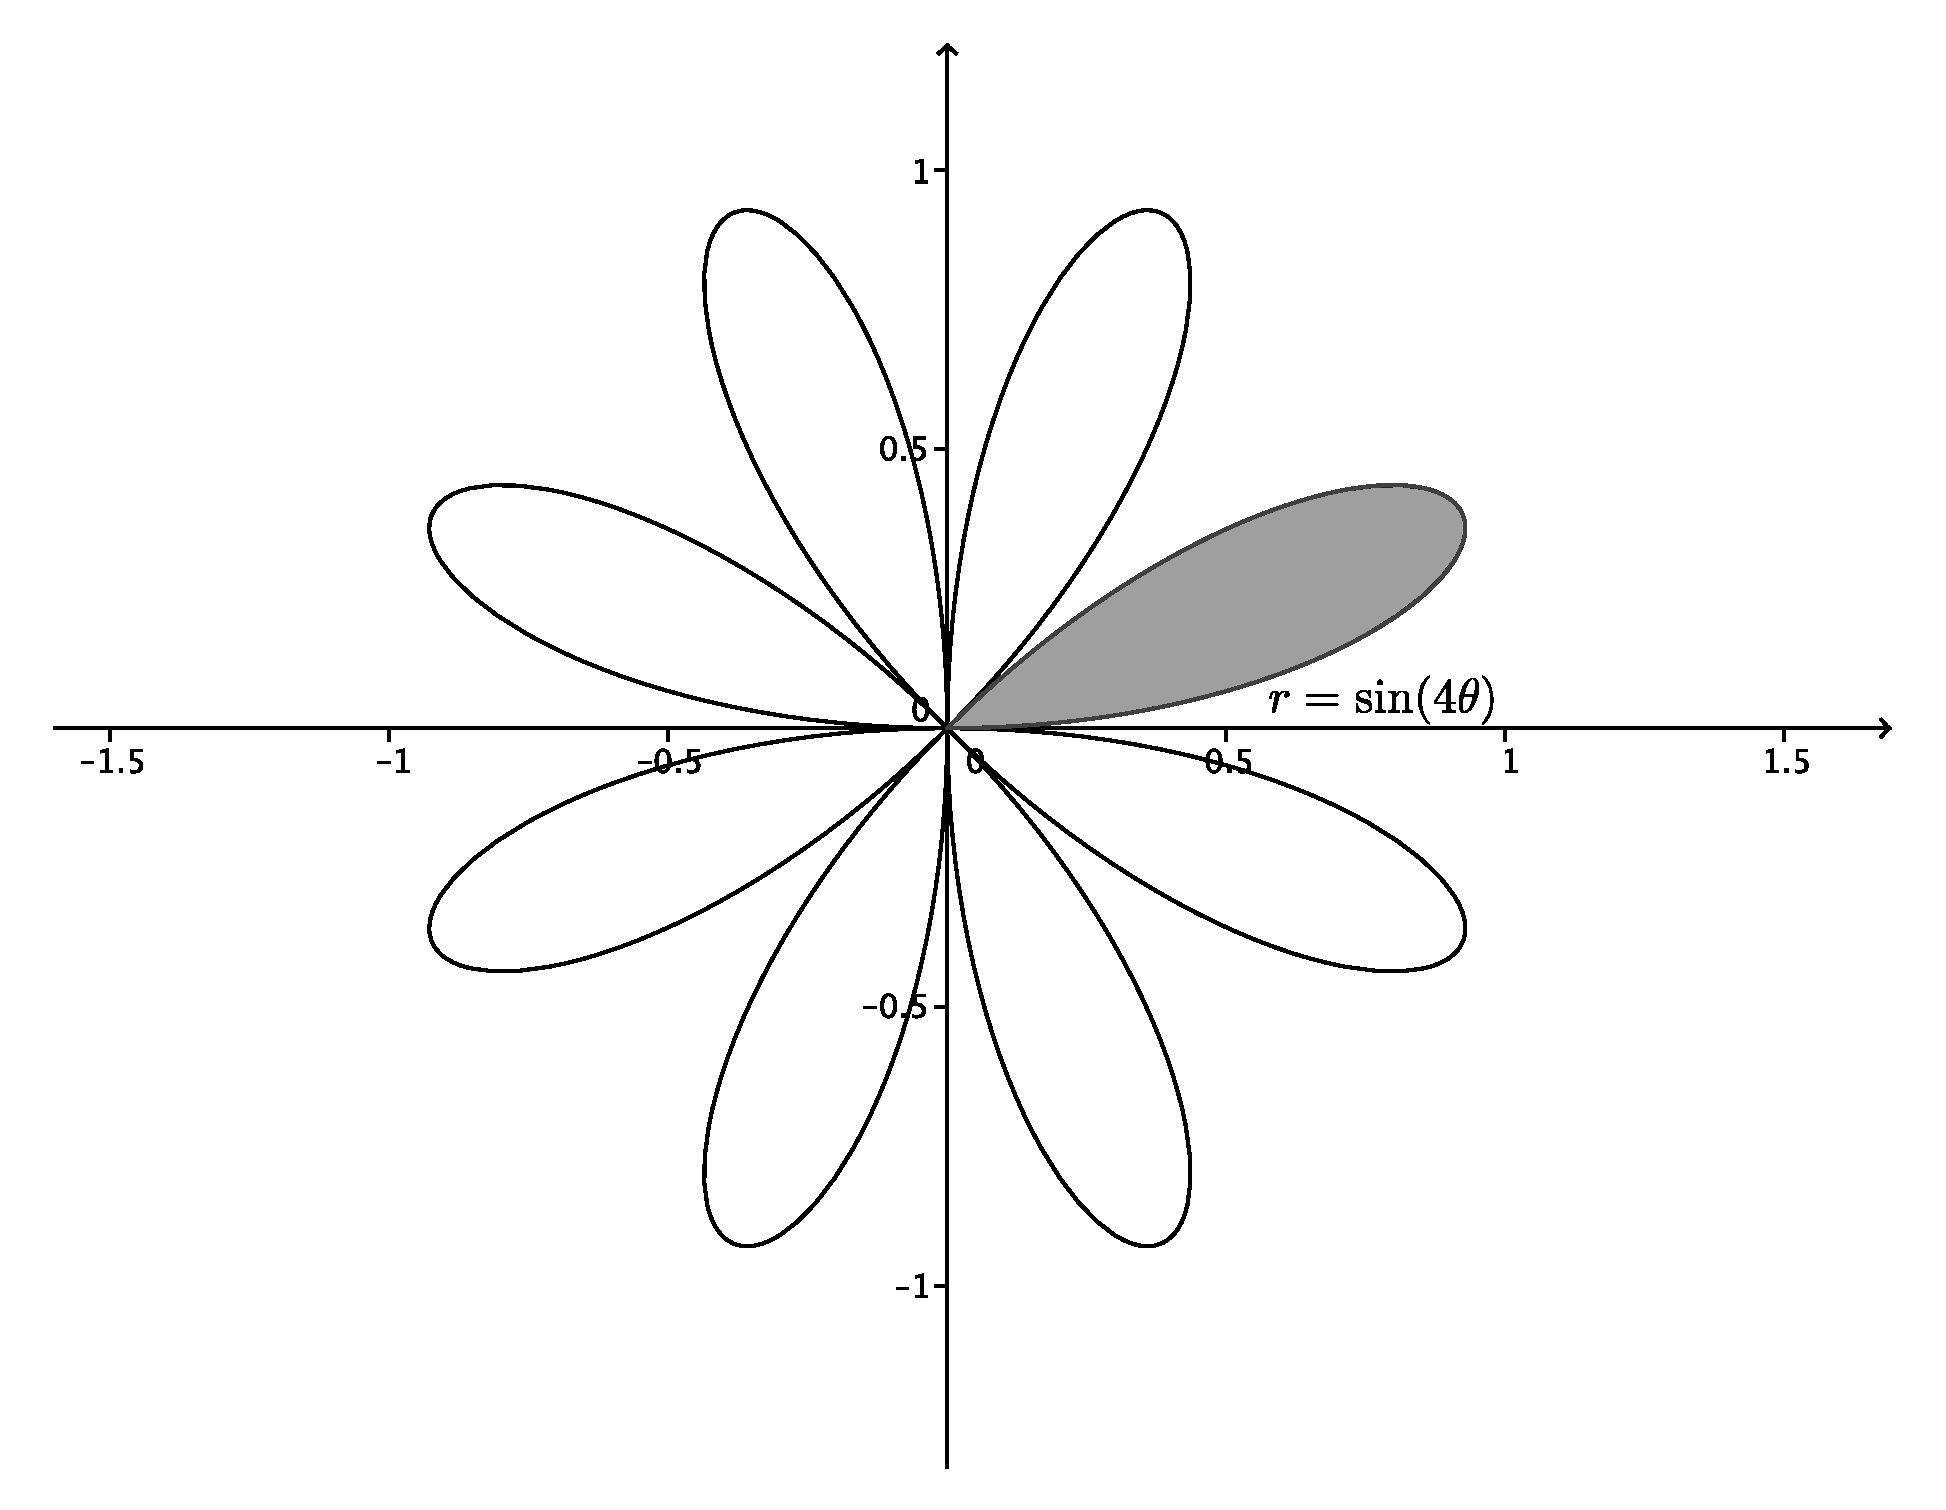
\includegraphics[width=0.9\columnwidth]{WS7-6c}

 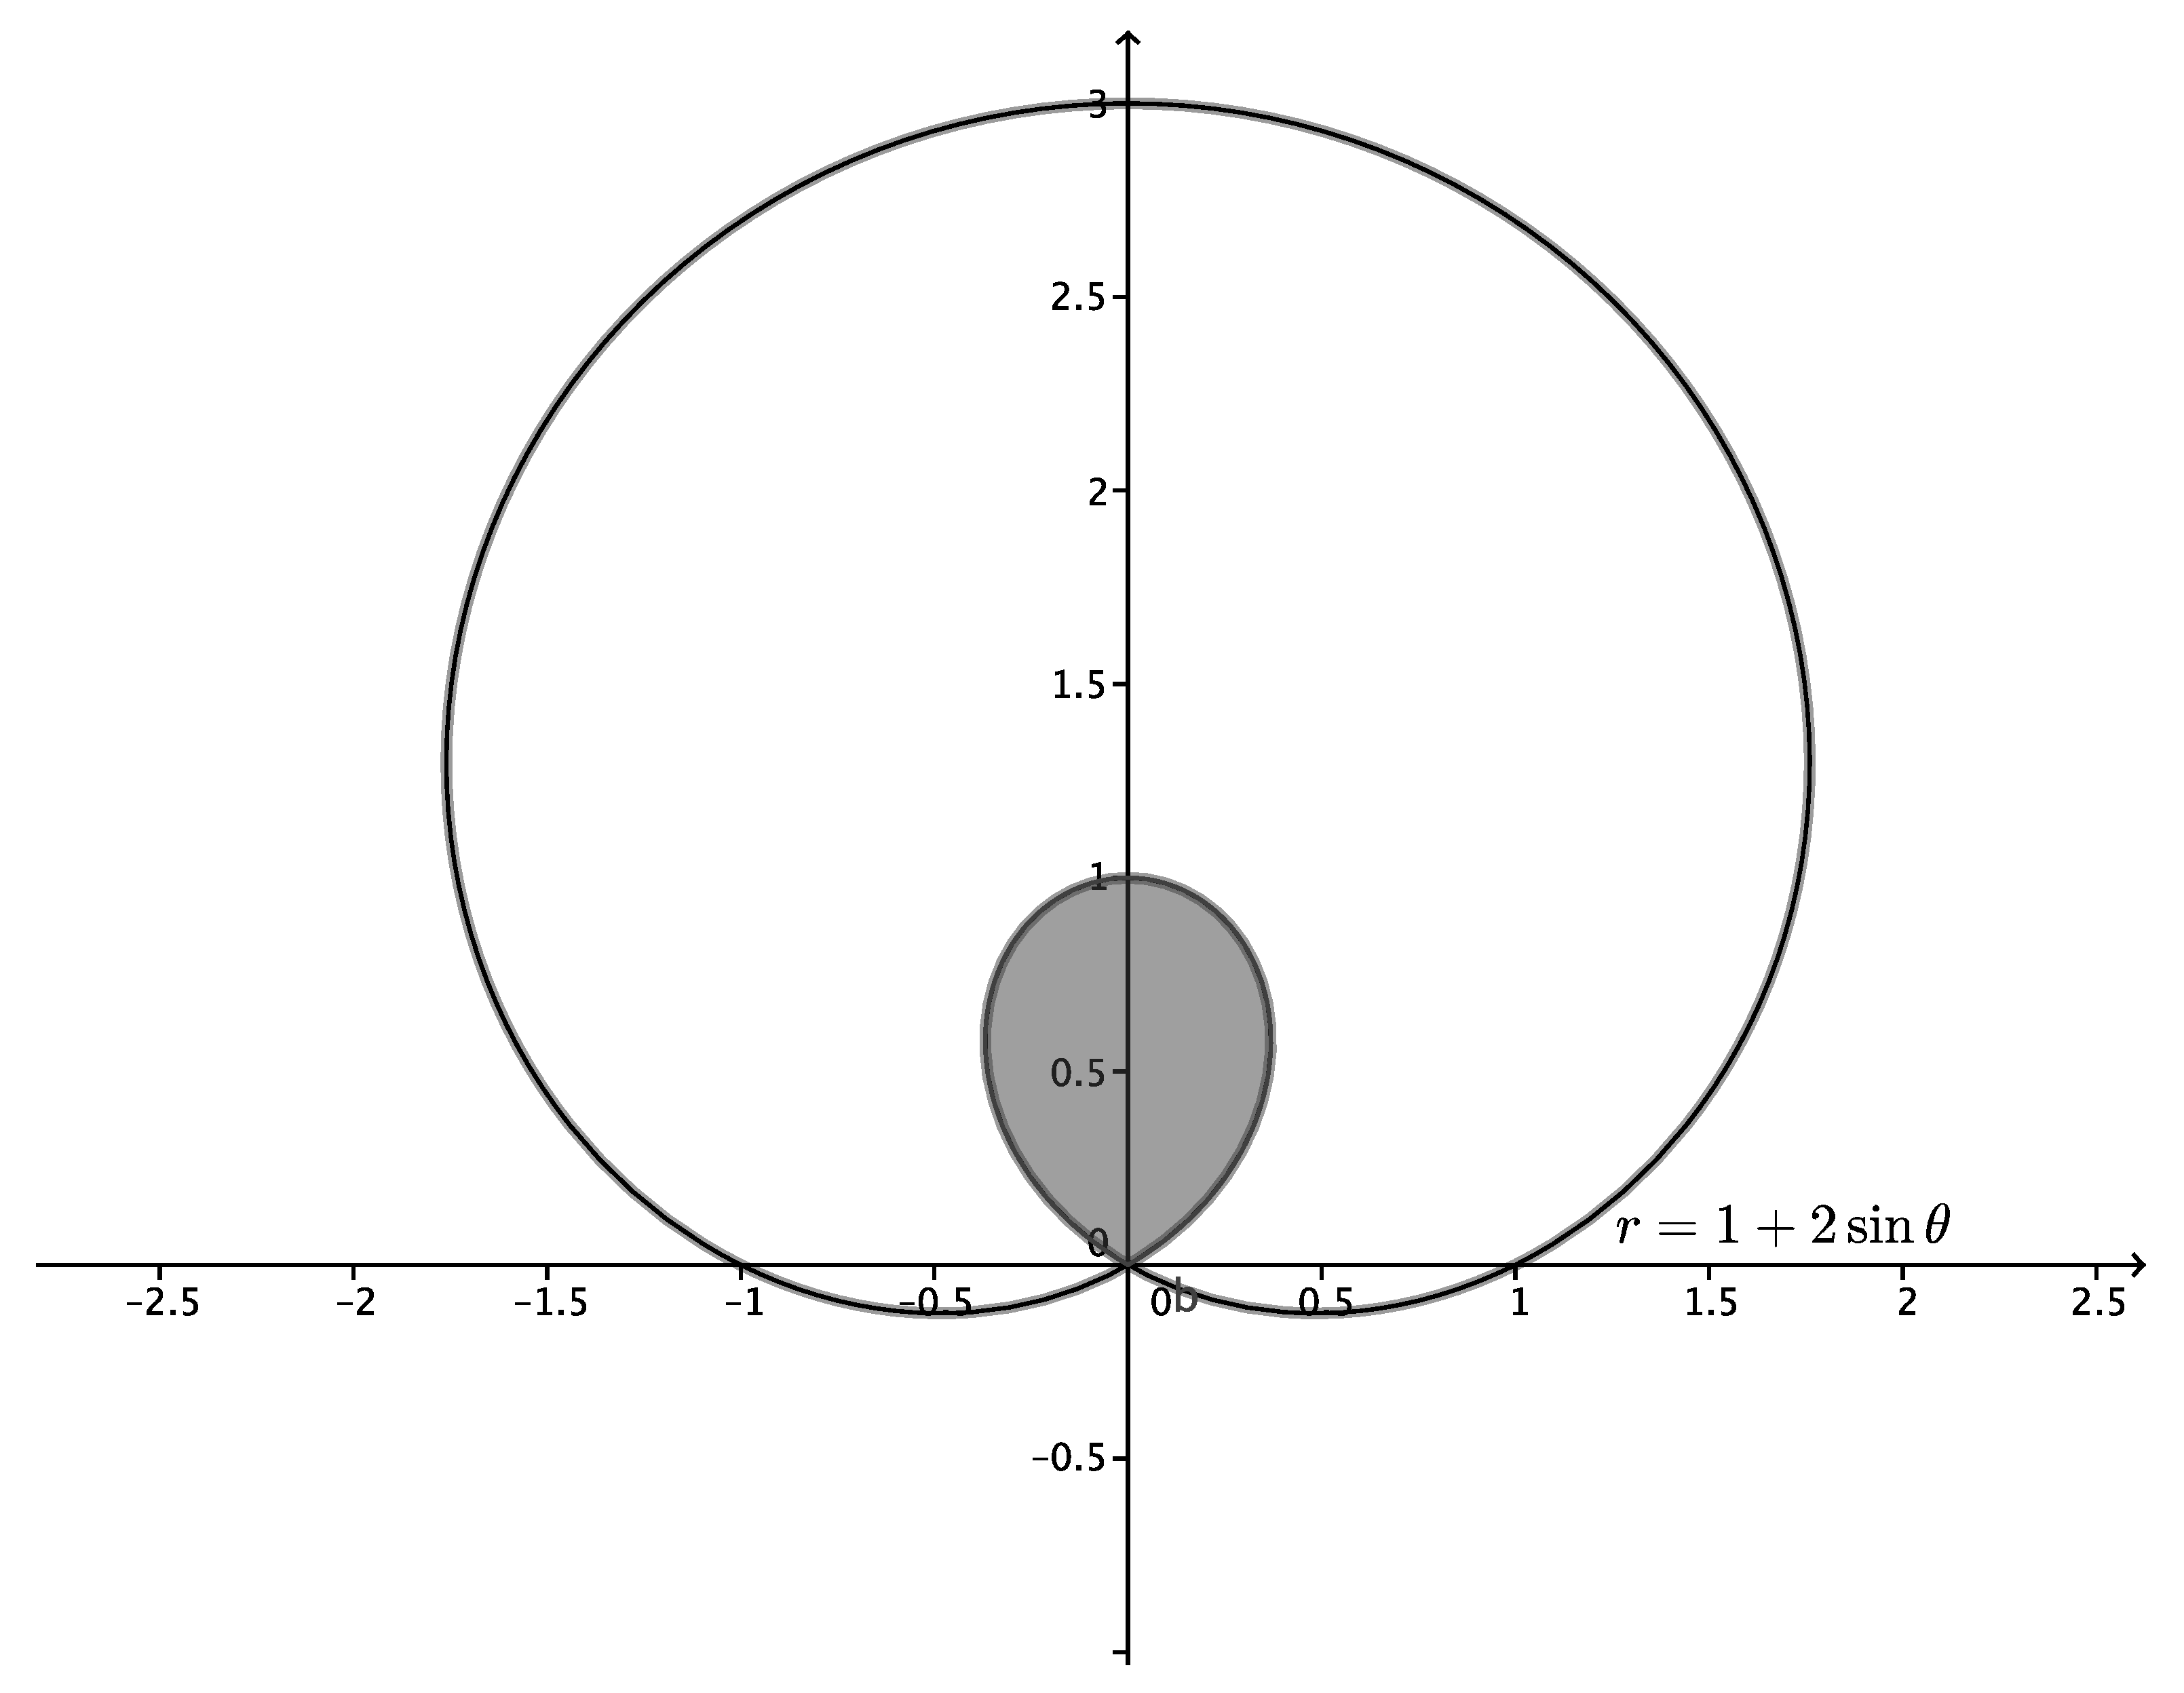
\includegraphics[width=0.9\columnwidth]{WS7-6d}

\end{multicols}


\end{enumerate}





\end{document}